\chapter{Example Meshes}

In the first chapter, we gave a brief introduction to mesh generation. We discussed structured, unstructured, simplical and non-simplical meshes and included a brief literature review of the research papers in the field of mesh generation. There, we stressed on the importance of generating anisotropic meshes or boundary layer meshes when solving for boundary layer phenomena and motivated the problem of generating stretched quad-dominant surface meshes to serve as the starting point of complete three dimensional anisotropic volume mesh generation.

We started discussing the method we developed to generate such anisotropic quad-dominant meshes in the second chapter. Here, we discussed the surface import, point placement, local reconnection and front recovery subroutines which are an essential part of the mesh generation process. In the third chapter, we discussed the subroutines used to advance several layers of the mesh and close off the marching layers so as to form a complete surface mesh. Controlling the aspect ratio on the advancing front, combining triangular elements to quadrilateral ones, mesh smoothing and collision handling were discussed.

In this chapter, we present some of the example meshes generated by using the Entire Domain Advancing Layer Surface Mesh Generator (EDAMSurf).


\section{Robustness Test 1 --- Concave Corners}

\begin{figure}
	\centering
	\begin{subfigure}{0.5\textwidth}
		\centering
		\includegraphics[width = 0.95\linewidth]{img/r/variousAngle-x0.5-g1.04/variousAngle.eps}
		\caption{}
		\label{fig-variousAngle-low}
	\end{subfigure}%
	\begin{subfigure}{0.5\textwidth}
		\centering
		\includegraphics[width=0.95\linewidth]{img/r/variousAngle-x0.3-g1.08/variousAngle.eps}
		\caption{}
		\label{fig-variousAngle-high}
	\end{subfigure}
	\begin{subfigure}{0.5\textwidth}
		\centering
		\includegraphics[width=0.95\linewidth]{img/r/variousAngle-x0.5-g1.04/corner.eps}
		\caption{}
		\label{fig-variousAngle-corner-low}
	\end{subfigure}%
	\begin{subfigure}{0.5\textwidth}
		\centering
		\includegraphics[width=0.95\linewidth]{img/r/variousAngle-x0.3-g1.08/corner.eps}
		\caption{}
		\label{fig-variousAngle-corner-high}
	\end{subfigure}
	\caption{Geometry with a variety of concave corners at the boundary is meshed with advancing layer surface mesh generation subroutine. On the left, the geometry is meshed with a growth ratio of 1.04 while on the right, it is meshed with a growth ratio of 1.08. The initial extrusion length of the mesh on the right is 40\% less than that on the left. (c) and (d) show the magnified view of a 30$^\circ$ concave corner corresponding to each of the meshes.}
	\label{fig-variousAngle}
\end{figure}

Generating a valid surface mesh for geometries with many concave corners is not a simple task. Vertices situated near a concave corner of the advancing layer encroach on each other, and there is very limited space available to march into. Hence, a robust collision handling subroutine is required to generate a valid mesh at such locations.

To illustrate the robustness of the advancing layer algorihtm, especially at the concave corners of the geometry, we run EDAMSurf on a geometry which has surfaces with a variety of concave corners at their boundaries. Figure \ref{fig-variousAngle} shows the resultant meshes generated on such a geometry for two growth ratios: 1.04 and 1.08. The geometry consists of a planar surface with six corners extruded normal to the surface. The concave corners on the geometry range from a 90$^\circ$ corner to a 30$^\circ$ corner.

\begin{figure}
	\centering
	\begin{subfigure}{0.5\textwidth}
		\centering
		\includegraphics[width=0.9\linewidth]{img/r/variousAngle-x0.5-g1.04/angleDistribution.pdf}
		\caption{}
		\label{fig-va-dist-low}
	\end{subfigure}%
	\begin{subfigure}{0.5\textwidth}
		\centering
		\includegraphics[width = 0.9\linewidth]{img/r/variousAngle-x0.3-g1.08/angleDistribution.pdf}
		\caption{}
		\label{fig-va-dist-high}
	\end{subfigure}
	\caption{Distribution of interior angles of the cells for the meshes generated for the geometry with a variety of concave corners (shown in figure \ref{fig-variousAngle}). Most of the angles are in 45$^\circ$-135$^\circ$ range with a very few skinny traingles.}
	\label{fig-variousAngle}
\end{figure}

Surface meshes generated from the geometry can be seen to have the required anisotropic elements at the boundary of the surface. Figure \ref{fig-variousAngle-corner-low} and \ref{fig-variousAngle-corner-high} show magnified view of a 30$^\circ$ concave corner in the mesh. Even though the mesh is advancing from the sharp corner towards the surface interior, it successfully recovers the front at each iteration of the advancing layer routine. Also, the quality of the mesh elements remains consistent as the mesh grows from the boundary. Additionally, the boundary topology is successfully retained several layers into the advancing layer mesh generation process. Hence, EDAMSurf is successful in marching out concave corners for the given geometry.

Figure \ref{fig-variousAngle} shows the distribution of interior angles of the mesh elements of these meshes. In this example, the majority of the angles in the mesh are around 90$^\circ$. The distribution is a bit flattened out. This is due to more concave corners in this geometry. Still, the number of skinny triangles in the mesh is negligible. The percentage of quads generated for the low growth ratio mesh is 96.43\% and for the high growth ratio mesh is 95.82\%. Hence, even though the mesh has many concave corners, more than 95\% of the mesh elements are non-simplical quad elements.

\section{Robustness Test 2 --- Diverse Topology Handling}

In the previous section, we saw how EDAMSurf is capable of meshing geometries with sharp corners. We test our advancing layer mesh generation subroutine for one more case. Here, we input a geometry which is shaped like a mechanical joint. The solid body has 10 surfaces. Each of the surface is different from the rest. There are curved as well as flat surfaces. The surfaces of the mechanical part test EDAMSurf with a variety of surface patches or segmented sub surfaces.

Figure \ref{fig-joint} shows the output mesh generated from the mechanical joint from several angles. Highly stretched elements are created at the boundary of the geometry. As the mesh grows towards the surface interior, the advancing layer grows in size, hence generating the required level of anisotropy at the boundaries. The aspect ratio for this mesh at the boundary varies with the boundary vertices but is set to be around 9-10. This illustrates that the mesh generator is capable of handling a variety of surface topologies. The mesh contains 45,740 cells and 45,020 points. There are 44,304 quadrilateral elements in the mesh while the number of triangular elements is just 1436.

\begin{figure}[hbt!]
	\centering
	\begin{subfigure}{.33\textwidth}
		\centering
		\includegraphics[width=.9\linewidth]{img/r/joint-x0.004-g1.04-a5/oblique.eps}
		\caption{}
		\label{fig-joint-oblique}
	\end{subfigure}%
	\begin{subfigure}{.33\textwidth}
		\centering
		\includegraphics[width=.9\linewidth]{img/r/joint-x0.004-g1.04-a5/oblique1.eps}
		\caption{}
		\label{fig-joint-oblique1}
	\end{subfigure}%
	\begin{subfigure}{.33\textwidth}
		\centering
		\includegraphics[width=.9\linewidth]{img/r/joint-x0.004-g1.04-a5/side.eps}
		\caption{}
		\label{fig-joint-side}
	\end{subfigure}
	\begin{subfigure}{.33\textwidth}
		\centering
		\includegraphics[width=.9\linewidth]{img/r/joint-x0.004-g1.04-a5/top.eps}
		\caption{}
		\label{fig-joint-top}
	\end{subfigure}%
	\begin{subfigure}{0.33\textwidth}
		\centering
		\includegraphics[width=0.9\linewidth]{img/r/joint-x0.004-g1.04-a5/front.eps}
		\caption{}
		\label{fig-joint-front}
	\end{subfigure}%
	\begin{subfigure}{0.33\textwidth}
		\centering
		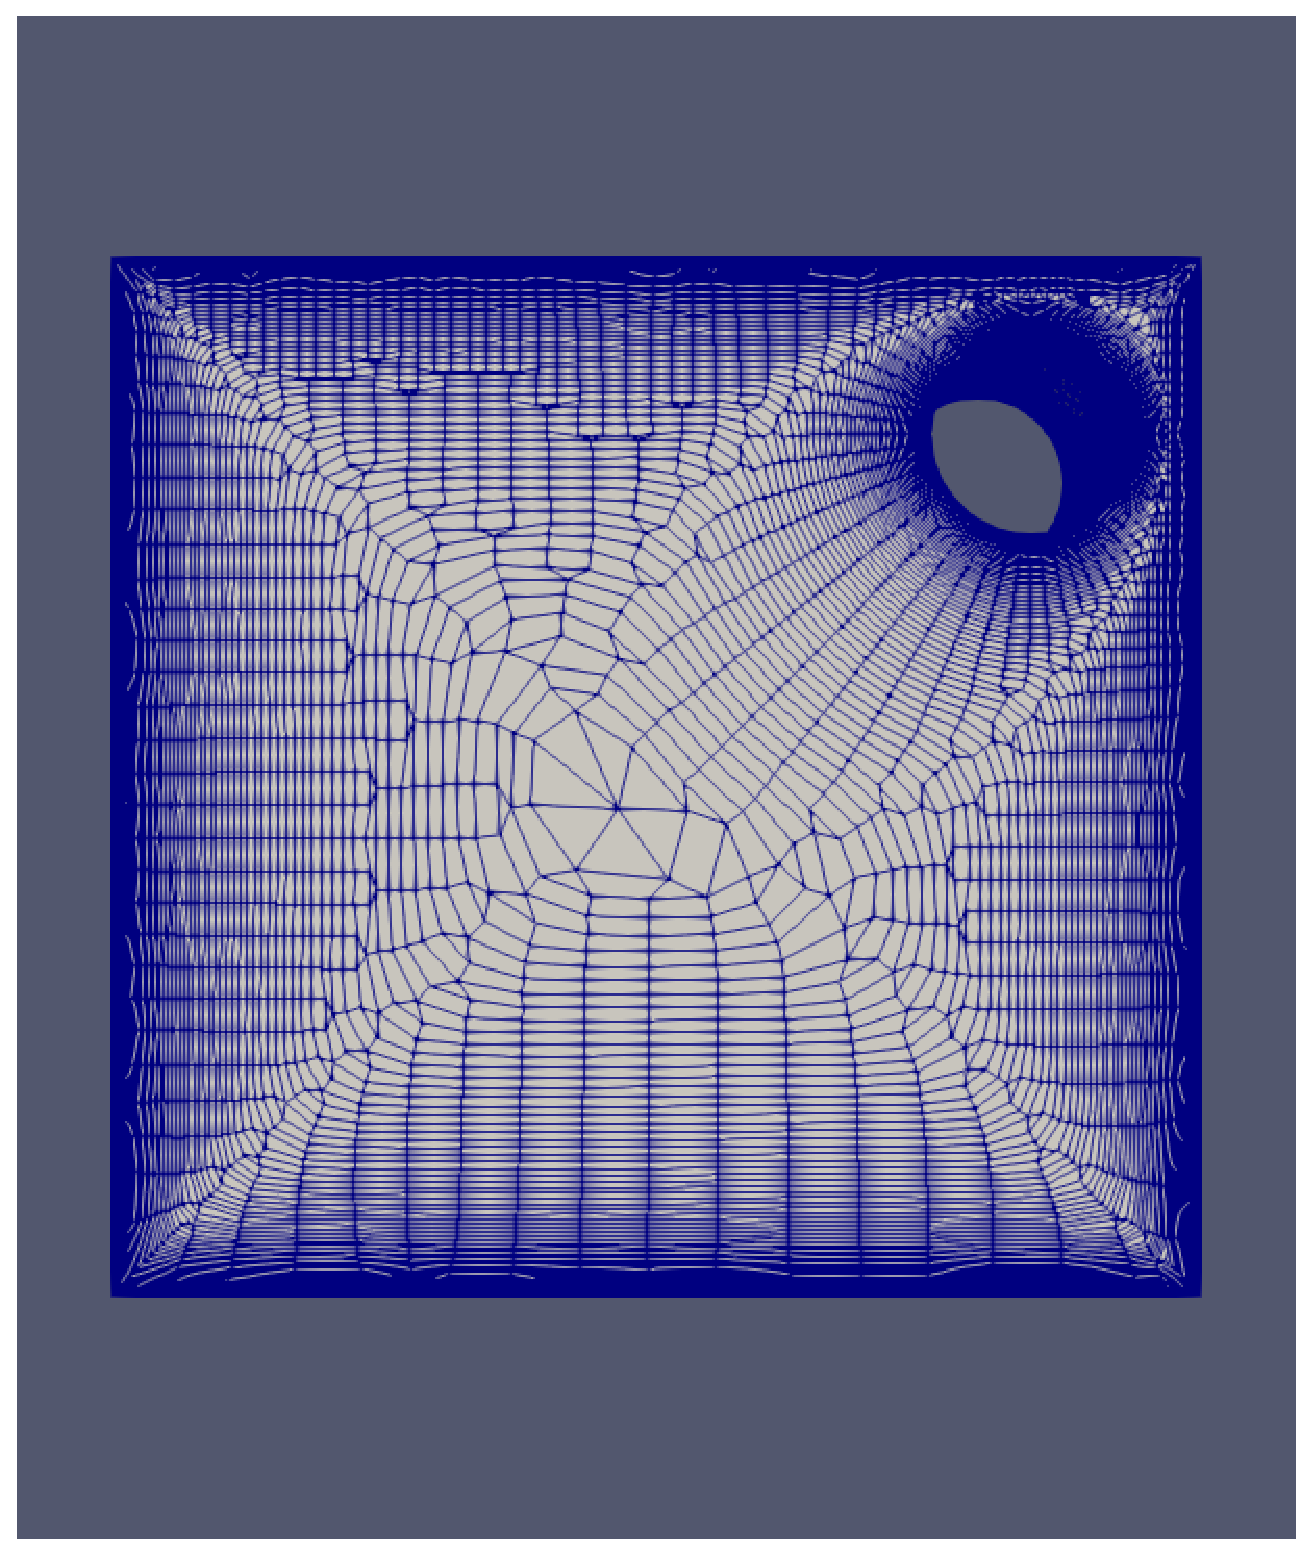
\includegraphics[width=0.9\linewidth]{img/r/joint-x0.004-g1.04-a5/bottom.eps}
		\caption{}
		\label{fig-joint-bottom}
	\end{subfigure}
	\caption{Geometry shown in Figure \ref{fig-surfSegment} is meshed using the advancing layer surface mesh generation routine. The algorithm is able to tackle a variety of surface topologies while generating anisotropic meshes. Given level of anisotropy can be obtained on the boundaries of the mesh with the algorithm.}
	\label{fig-joint}
\end{figure}

In Figure \ref{fig-closeUp}, we show close-ups at two locations on the mesh where advancing layers from several boundaries collide in a comparatively limited region. Figure \ref{closeUp1} shows the close up view of the top of the mechanical part, near the region where the flat section with a cylindrical cutout meets the curved surface at the top. Advancing layers from the circular boundary of the cylindrical cutout and the two straight boundaries of the surface path collide after advancing several layers onto the surface. At each advancing layer, collision handling subroutine checks for possible encroaching vertices. It stops selected points from marching forward to avoid front collapse and hence finishes the mesh generation process in some regions of the surface patch while continuing the process in the remaining regions.

Another example of collision between multiple independently advancing marching layers on the surface mesh is shown in figure \ref{closeUp2}. Here, we show the bottom of the mechanical part near the cylindrical cutout. Layers start to march from the circular cutout as well as the rectangular boundary of the bottom surface. There is high anisotropy at these boundary curves. As the layers march onto the surface, we see that the aspect ratio of the mesh elements gradually drops. One by one, the points on an advancing front which encroach on other points are stopped from marching. This is done until the point when there are no more vertices left on the advancing front to march futher. This completes the mesh generation process. These figures demonstrates the robustness of EDAMSurf. Hence, it is possible to mesh a surface with varied topological features using our mesh generation scheme.

\begin{figure}
	\centering
	\begin{subfigure}{.5\textwidth}
		\centering
		\includegraphics[width=0.9\linewidth]{img/r/joint-x0.004-g1.04-a5/closeUp.eps}
		\caption{}
		\label{closeUp1}
	\end{subfigure}%
	\begin{subfigure}{.5\textwidth}
		\centering
		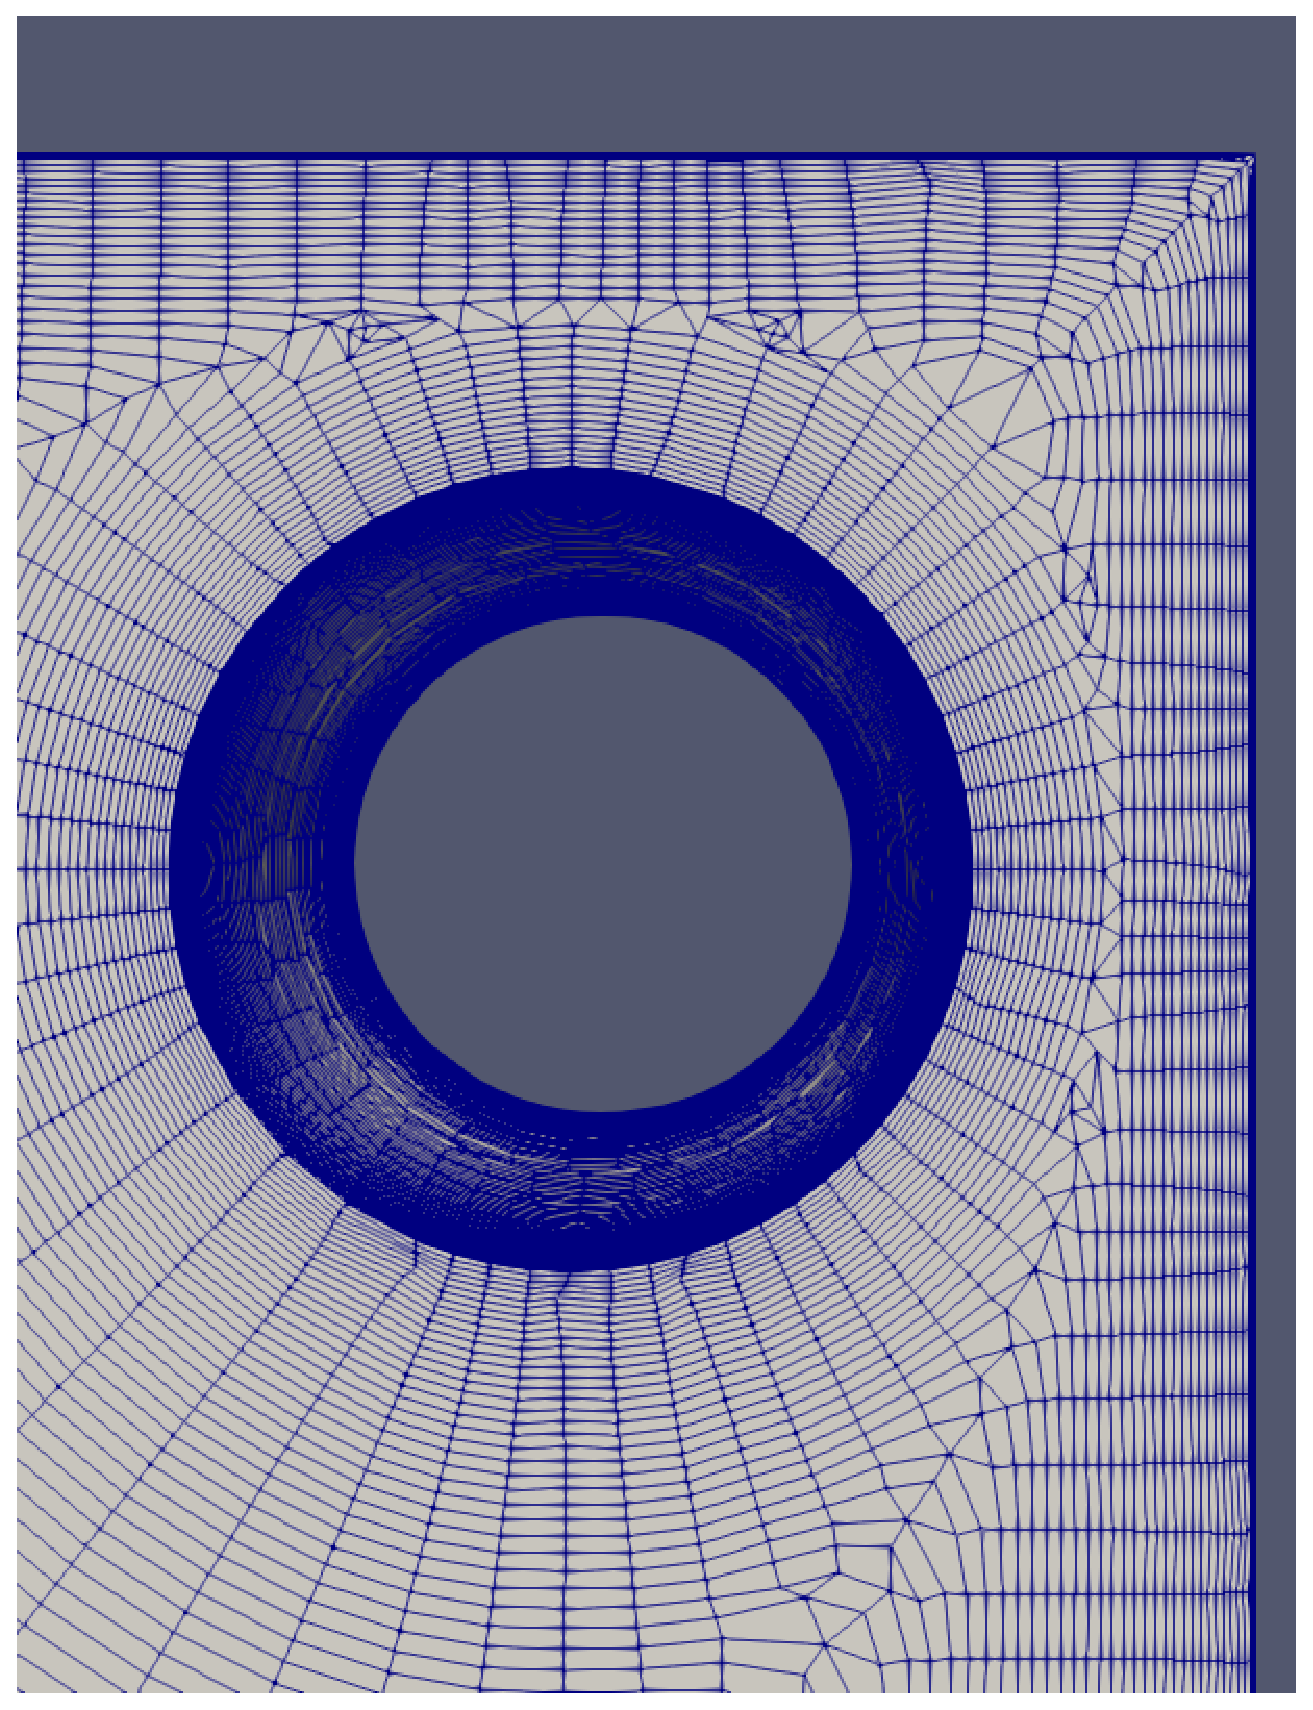
\includegraphics[width=0.9\linewidth]{img/r/joint-x0.004-g1.04-a5/bottomCloseUp.eps}
		\caption{}
		\label{closeUp2}
	\end{subfigure}
	\caption{Close up views of the meshes generated from mechanical joint. (a) Close up view of from the top of the mechanical joint as seen in Figure \ref{fig-joint-top}, near the region where the flat section with a cylindrical cutout meets the curved surface at the top. (b) Bottom of the part near the cylindrical cut out. Mesh layers collide at various angles in these examples. The advancing front stops marching some of its vertices using the collision handling subroutine and the algorithm continues to march the next layer on to the remaining region on the surface.}
	\label{fig-closeUp}
\end{figure}

\section{NACA0018}

In the previous two sections, we saw how EDAMSurf is capable geometries with sharp corners and diverse topology. In this section, we try to mesh a simple airfoil geometry. We take the NACA0018 airfoil 2D profile and extrude it in 3D. The ends of the airfoil are closed by a flat surface with the NACA0018 profile as its boundary curve. This gives us a three dimensional airfoil as shown in the Figure \ref{fig-naca0018}. The chord length of the airfoil is 1 and the span is 6. After generating a triangulation from the solid body using the freely available software MeshLab \cite{LocalChapterEvents:ItalChap:ItalianChapConf2008:129-136}, we import it to EDAMSurf. We mesh the geometry using our advancing layer surface mesh generation routine. The airfoil profile is segmented into four sub surfaces. Two surfaces represent the two ends of the airfoil while the other two represent the top and the bottom of the airfoil.

\begin{figure}
	\centering
	\includegraphics[width=0.6\linewidth]{img/r/naca0018.png}
	\caption{NACA0018 Airfoil profile extruded along the normal direction.}
	\label{fig-naca0018}
\end{figure}

\begin{figure}
	
	\centering
	
	\begin{subfigure}{0.4\textwidth}
		\centering
		\includegraphics[width = 0.9\linewidth, trim={0 7cm  0 7cm},clip]{img/r/naca0018-x0.007-g1.05/endCap.eps}
		\caption{}
		\label{fig-endCap-low}
	\end{subfigure}%
	\begin{subfigure}{0.4\textwidth}
		\centering
		\includegraphics[width=0.9\linewidth,trim={0 7cm  0 7cm},clip]{img/r/naca0018-x0.007-g1.1/endCap.eps}
		\caption{}
		\label{fig-endCap-high}
	\end{subfigure}
	
	\begin{subfigure}{0.4\textwidth}
		\centering
		\includegraphics[width=0.9\linewidth]{img/r/naca0018-x0.007-g1.05/oblique.eps}
		\caption{}
		\label{fig-oblique-low}
	\end{subfigure}%
	\begin{subfigure}{0.4\textwidth}
		\centering
		\includegraphics[width=0.9\linewidth]{img/r/naca0018-x0.007-g1.1/oblique.eps}
		\caption{}
		\label{fig-oblique-high}
	\end{subfigure}%
	\caption{NACA0018 airfoil meshed with our advancing layer surface mesh algorithm. Meshes shown on the left ((a) and (c)) correspond to a growth ratio of 1.05 while ones shown on the right ((b) and (d) correspond to a growth ratio of 1.1. Anisotropic refinement of the mesh can be seen at the leading edge, trailing edge, and both end caps of the airfoil.}
	\label{fig-naca}
\end{figure}

We show two of the meshes we generate from this geometry. The first one is shown in Figure \ref{fig-endCap-low} and \ref{fig-oblique-low}. Here, we use a growth ratio of 1.05 and an initial extrusion length of 0.007. The aspect ratio value at the boundary curves ranges from 5-25. The second mesh is shown in Figure \ref{fig-endCap-high} and \ref{fig-oblique-high}. The meshes can be seen to have anisotropic refinement at the leading edge, the trailing edge and at the boundary of the end caps of the airfoil. The discretization of the boundary of the airfoil is carried several layers into the surface mesh.

\begin{table}[]
	\caption{\label{table-naca} Mesh parameters for NACA0018 Airfoil (chord length $c = 1$)}
	\centering
	\begin{tabular}{c|c|c|c|c|c}\hline
		\begin{tabular}[c]{@{}c@{}}extrusion \\ length\end{tabular} & \begin{tabular}[c]{@{}c@{}}growth \\ ratio\end{tabular} & \begin{tabular}[c]{@{}c@{}}number\\ of quads\end{tabular} & \begin{tabular}[c]{@{}c@{}}number\\ of tris \end{tabular} & \% quads & \begin{tabular}[c]{@{}c@{}}\% angles\\ between 45$^{\circ}$-135$^{\circ}$\end{tabular} \\ \hline
		0.007                                                       & 1.05                                                    & 3750                                                     & 162                                                      & 95.86 & 97.38                                                              \\
		0.007                                                       & 1.1                                                     & 2678                                                      & 198                                                       & 93.11 & 96.22               \\                                               
		\hline
	\end{tabular}
\end{table}

In the meshes generated by EDAMSurf, most of the elements are quadrilateral elements. A very few triangular elements are also present in the mesh. As discussed in \ref{sec-simplicial}, these triangular elements help conform to the geometry while giving more flexibility during the mesh generation process.

\begin{figure}[!hbt]
	\centering
	\begin{subfigure}{0.5\textwidth}
		\centering
		\includegraphics[width=0.9\linewidth]{img/r/naca0018-x0.007-g1.05/angleDistribution.pdf}
		\caption{}
		\label{fig-dist-low}
	\end{subfigure}%
	\begin{subfigure}{0.5\textwidth}
		\centering
		\includegraphics[width = 0.9\linewidth]{img/r/naca0018-x0.007-g1.1/angleDistribution.pdf}
		\caption{}
		\label{fig-dist-high}
	\end{subfigure}
	\caption{Distribution of interior angles of the cells for the meshes generated for NACA 0018 airfoil. Most of the angles of the cells in the mesh are around 90$^\circ$ with a very few skinny angles.}
	\label{fig-angle-distribution}
\end{figure}

Table \ref{table-naca} shows the mesh parameters for the two cases shown in the figure. In the higher growth ratio case, 96.22\% of the angles in the mesh elements are between 45$^\circ$ and 135$^\circ$. In the mesh with the lower growth ratio, 97.38\% of the angles are in that range. In Figure \ref{fig-angle-distribution}, we plot the distribution of angles for the mesh elements in the two meshes. As can be seen from the distribution, for both the cases, most of the angles are withing a 30$^\circ$ range of 90$^\circ$. The distribution is plotted on a log scale to highlight the variation from the mean value. The distribution of angles is more spread out for the higher growth ratio case due to a higher number of triangles in that case. A small fraction of the angles is close to 0$^\circ$ and 180$^\circ$. This is because of the sharp trailing edge of the geometry, which has to be dealt with using the corner collision algorithm described in section \ref{collisionConcaveCorner}. Overall, the algorithm produces quad dominant meshes with a very few skinny cells.

This NACA0018 airfoil example shows that EDAMSurf can create stretched or anisotropic meshes for simple airfoil geometries. It produces a mesh consisting primarily of quadrilateral elements with a few triangular elements. Lastly, the topology of the boundary curves of the sub surfaces is propagated several layers into the mesh.

